\chapter{Identificación de Requisitos}

\begin{figure}[H] 
    \caption{\doublespacing \\ \textit{Comparación de los modelos de fusión desde lightweight hasta Large.}} 
    \centering
    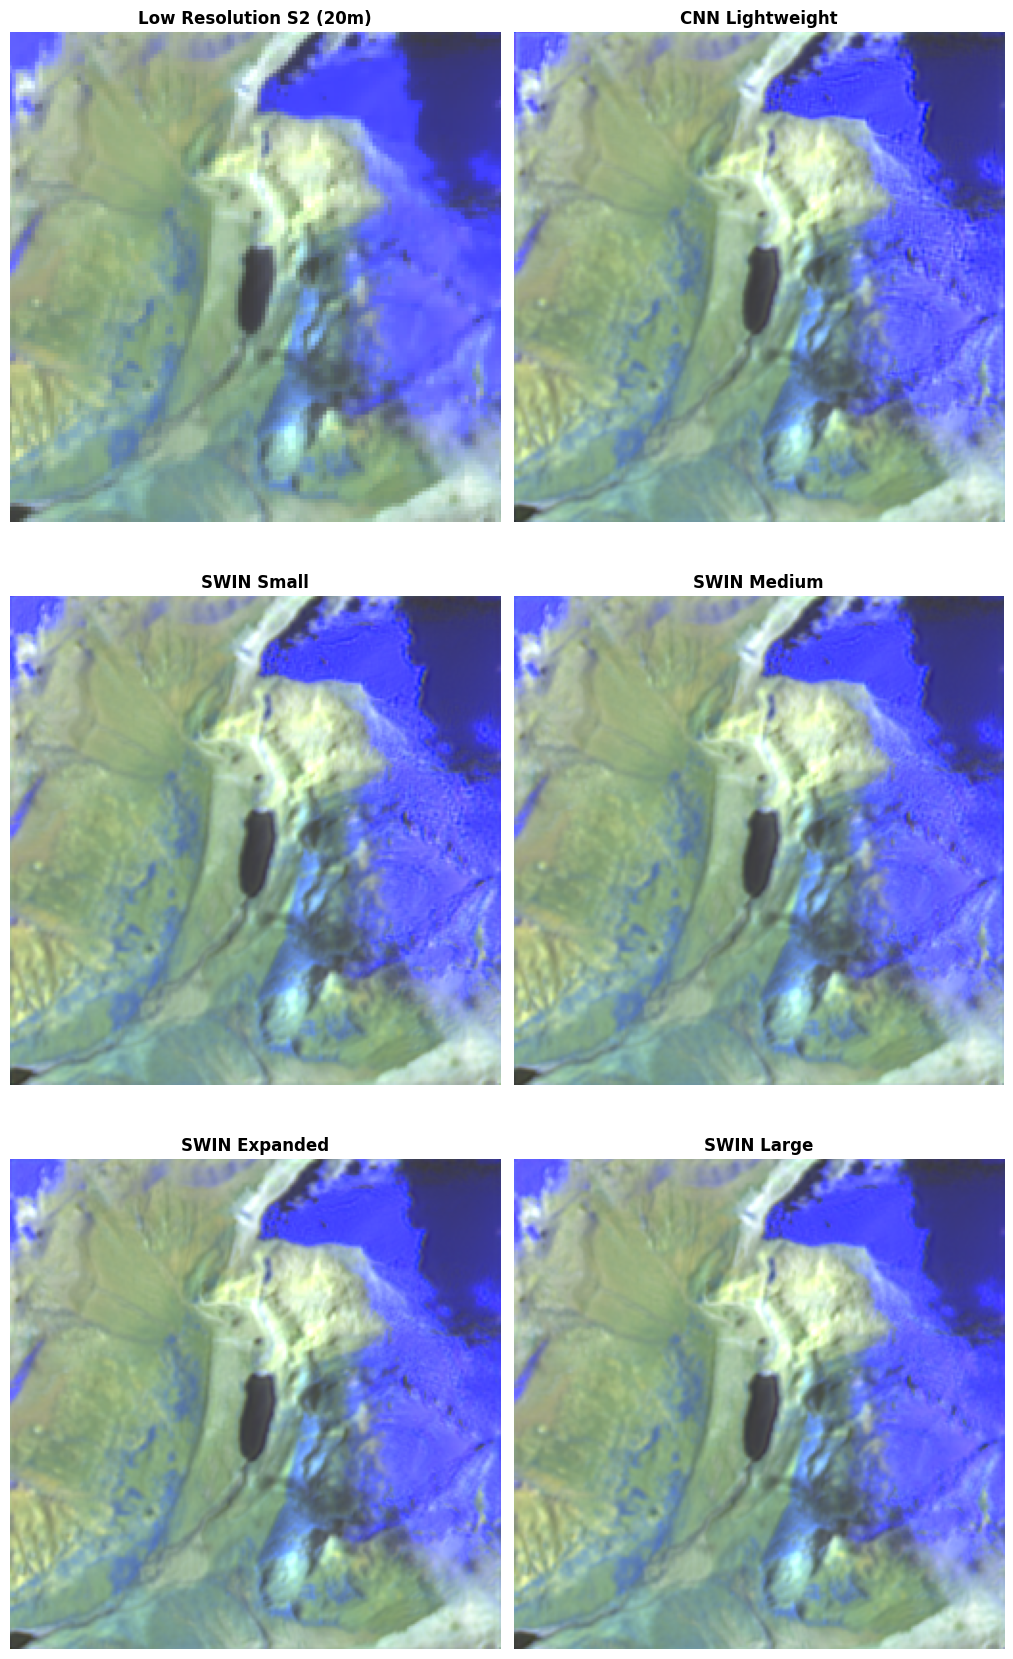
\includegraphics[width=1\linewidth]{images/results10m.png}
    \begin{justify}
        \textit{Nota.} Esquema que muestra la preparación de datos y el modelo de Fusión x2, donde las bandas de entrada son ajustadas en resolución para generar una salida unificada de 20 metros, combinando detalles espaciales y espectrales. Elaboración propia.
    \end{justify}                    
    \label{fig:fusionx2_training}
\end{figure}
\section{Trabajo Previo Realizado}
En este capítulo se describe el trabajo previo realizado para guiar el desarrollo del software, considerando la identificación del problema y el contexto habitual de uso o funcionamiento de la aplicación.

\subsection{Identificación del Problema}
Uno de los principales retos en el análisis de imágenes satelitales es la falta de sensores de alta resolución de acceso abierto. Esto limita la capacidad de realizar estudios detallados y precisos en diversas aplicaciones geoespaciales.

\subsection{Contexto de Uso}
El software desarrollado está diseñado para funcionar en entornos de inferencia, donde se espera que procese imágenes satelitales y aplique técnicas de superresolución en tiempo real o en procesos de análisis. La identificación de requisitos ha sido realizada en conjunto con expertos en la materia para asegurar su aplicabilidad y eficiencia en escenarios reales de teledetección.

\chapter{Descripción de la Herramienta Software Desarrollada}

\section{Detalles del Proceso de Desarrollo}
Este capítulo detalla el proceso de desarrollo del software, incluyendo las fases, los hitos alcanzados y los diagramas explicativos de la arquitectura y funcionamiento del modelo de superresolución.

\subsection{Fases del Desarrollo}
El desarrollo de la herramienta se dividió en fases clave, cada una con objetivos específicos:
\begin{itemize}
    \item \textbf{Fase de Planificación}: Identificación de requerimientos y objetivos.
    \item \textbf{Fase de Diseño}: Estructuración del modelo SR (Superresolución) y diseño de arquitectura.
    \item \textbf{Fase de Implementación}: Desarrollo de los módulos y entreno del modelo de superresolución.
    \item \textbf{Fase de Pruebas}: Validación y ajuste de parámetros para garantizar precisión y rendimiento.
\end{itemize}

\subsection{Diagramas de Flujo y Arquitectura}
Se presentan diagramas de flujo y arquitecturas que ilustran el funcionamiento del programa, explicando cada etapa del procesamiento y superresolución de imágenes. Estos diagramas proporcionan una visión clara de la estructura interna y la secuencia de operaciones.

\subsection{Capturas de Pantalla}
Para facilitar la comprensión del programa, se incluyen capturas de pantalla que muestran la interfaz de usuario y el proceso de superresolución, permitiendo al lector visualizar el flujo y resultado del programa.

\chapter{Evaluación}

\section{Usabilidad de la Herramienta}
La evaluación de la herramienta incluye una valoración de su usabilidad, centrada en la accesibilidad y eficiencia de la interfaz y su adaptabilidad para distintos usuarios en el ámbito de la teledetección.

\section{Aplicabilidad al Problema Propuesto}
Se analiza la aplicabilidad de la herramienta al problema de mejorar la resolución de imágenes satelitales. Este análisis se realiza con la colaboración de usuarios expertos, quienes evalúan la capacidad del modelo para ofrecer soluciones viables y de alta resolución en el contexto de aplicaciones geoespaciales avanzadas.
